% Created 2017-02-20 Mon 17:54
% Intended LaTeX compiler: pdflatex
\documentclass[presentation]{beamer}
\usepackage[utf8]{inputenc}
\usepackage[T1]{fontenc}
\usepackage{graphicx}
\usepackage{grffile}
\usepackage{longtable}
\usepackage{wrapfig}
\usepackage{rotating}
\usepackage[normalem]{ulem}
\usepackage{amsmath}
\usepackage{textcomp}
\usepackage{amssymb}
\usepackage{capt-of}
\usepackage{hyperref}
\usetheme{default}
\author{Petr Blaho}
\date{\today}
\title{PA200 - Cloud Computing Concepts}
\hypersetup{
 pdfauthor={Petr Blaho},
 pdftitle={PA200 - Cloud Computing Concepts},
 pdfkeywords={},
 pdfsubject={},
 pdfcreator={Emacs 25.1.1 (Org mode 9.0.5)}, 
 pdflang={English}}
\begin{document}

\maketitle


\begin{frame}[label={sec:org3e99d5e}]{Virtualization}
\begin{block}{Why?}
\begin{itemize}
\item Consolidation of resources
\item Virtual vs Physical machine inspection
\item Easy provisioning
\item Movable resource
\end{itemize}
\end{block}

\begin{block}{Why?}
\begin{itemize}
\item Recoverable
\item Easier testing and evaluation
\item Duplication of environments
\item Isolation from host HW and OS
\end{itemize}
\end{block}
\end{frame}

\begin{frame}[label={sec:orgb18dce3}]{Hypervisors}
\begin{itemize}
\item native
\item hosted
\end{itemize}
\begin{block}{Hypervisors}
\begin{center}
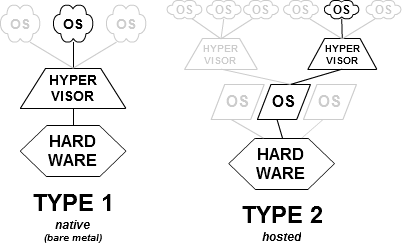
\includegraphics[width=.9\linewidth]{./hyperviseur.png}
\end{center}
\end{block}
\end{frame}

\begin{frame}[label={sec:orgab3aedb}]{Examples of native hypervisors}
\begin{itemize}
\item XEN
\item MS Hyper-V
\item VMware ESXi
\end{itemize}
\end{frame}

\begin{frame}[label={sec:orgd3a5b89}]{Examples of hosted hypervisors}
\begin{itemize}
\item QEMU
\item KVM
\item VirtualBox
\item VMware Workstation
\end{itemize}
\end{frame}

\begin{frame}[label={sec:orge3b530b}]{XEN}
\begin{itemize}
\item founded in 2003 by XenSource, bought in 2007 by Citrix
\item 2013 under Linux Foundation as Xen Project
\item native hypervisor
\end{itemize}
\end{frame}
\begin{frame}[label={sec:orgd3d44c5}]{ZEN}
\begin{center}
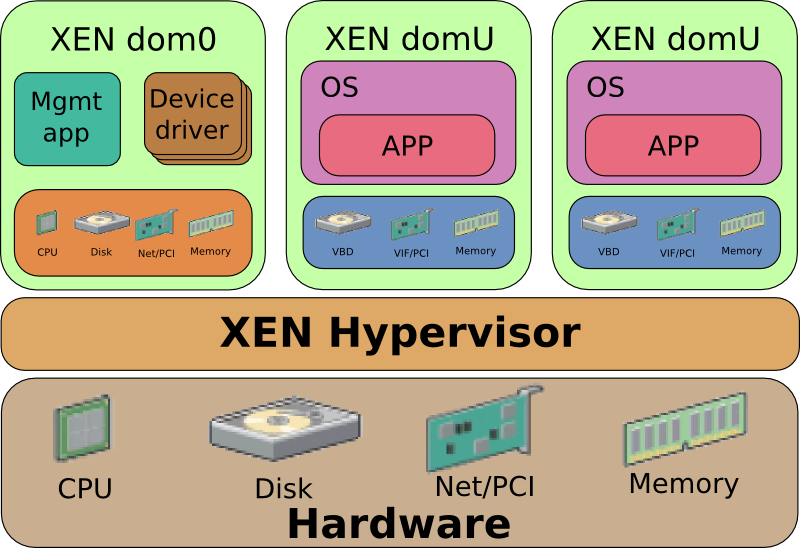
\includegraphics[width=.9\linewidth]{./xen.png}
\end{center}
\end{frame}

\begin{frame}[label={sec:orge81c349}]{KVM}
\begin{itemize}
\item Modular kernel virtualization
\item provides user space access to hw virtualization
\item started by Qumranet
\item 2007 merged into linux kernel
\end{itemize}
\end{frame}
\begin{frame}[label={sec:orge074f98}]{KVM}
\begin{center}
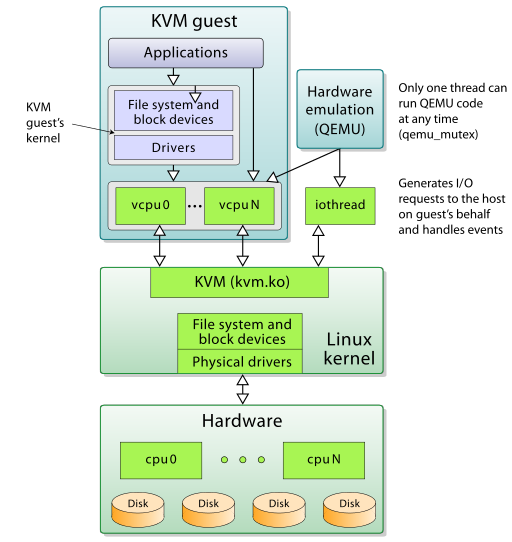
\includegraphics[width=.9\linewidth]{./kvm.png}
\end{center}
\end{frame}

\begin{frame}[label={sec:orgbcadd30}]{QEMU}
\begin{itemize}
\item hosted hypervisor
\item provides emulation of hw
\item can be used with KVM for hw virtualization
\end{itemize}
\end{frame}

\begin{frame}[label={sec:orgb278c22}]{Libvirt}
\begin{itemize}
\item Common API for hypervisor type abstraction
\item supports
\item LXC
\item KVM/QEMU, Xen, VirtualBox
\item VMware ESXi and Workstation
\item MS Hyper-V, IBM PowerVM
\end{itemize}
\end{frame}
\begin{frame}[label={sec:org14b5d67}]{Libvirt}
\begin{center}
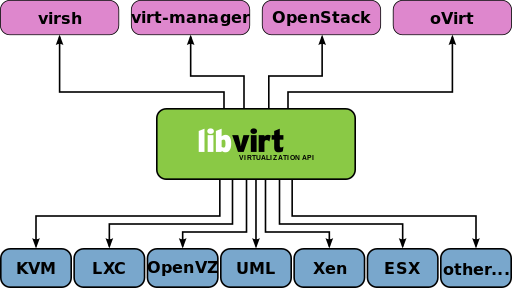
\includegraphics[width=.9\linewidth]{./libvirt.png}
\end{center}
\end{frame}

\begin{frame}[label={sec:orgacb4f67}]{oVirt}
\begin{itemize}
\item virtualization management platform
\item on top of KVM
\item upstream for RHV
\item engine
\item node
\item VDSM - virtual desktop and server manager
\end{itemize}
\end{frame}

\begin{frame}[label={sec:orgccd6ca5}]{OpenStack}
\begin{itemize}
\item software platform for cloud computing
\item started in 2010 by Rackspace and NASA
\item in 2012 founded OpenStack Foundation
\end{itemize}
\end{frame}
\begin{frame}[label={sec:orgd42efb4}]{OpenStack}
\begin{center}
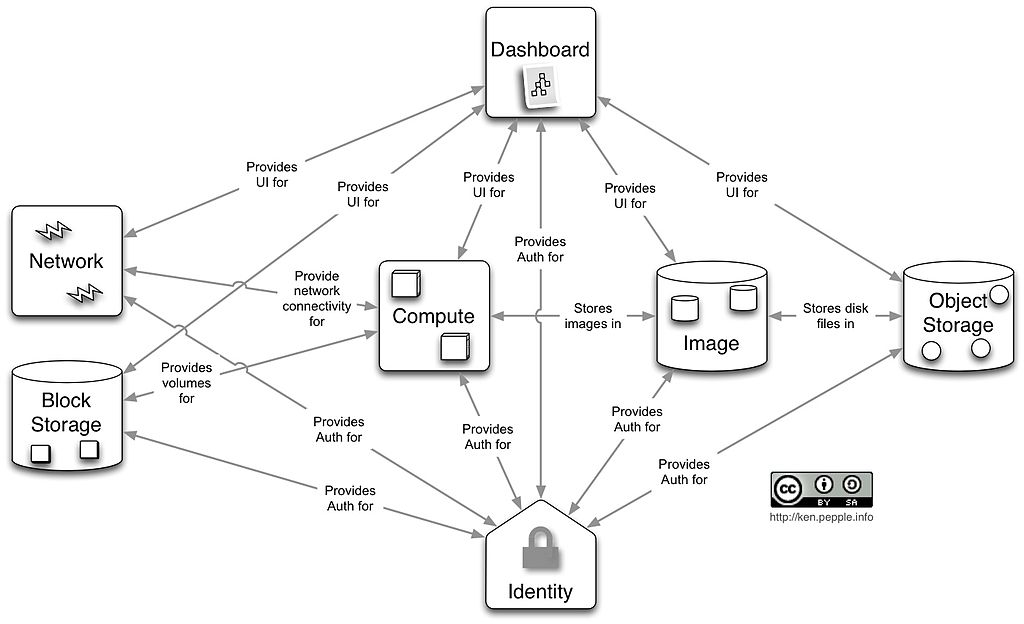
\includegraphics[width=.9\linewidth]{./openstack.jpg}
\end{center}
\end{frame}
\begin{frame}[label={sec:org04e2435}]{OpenStack}
\begin{center}
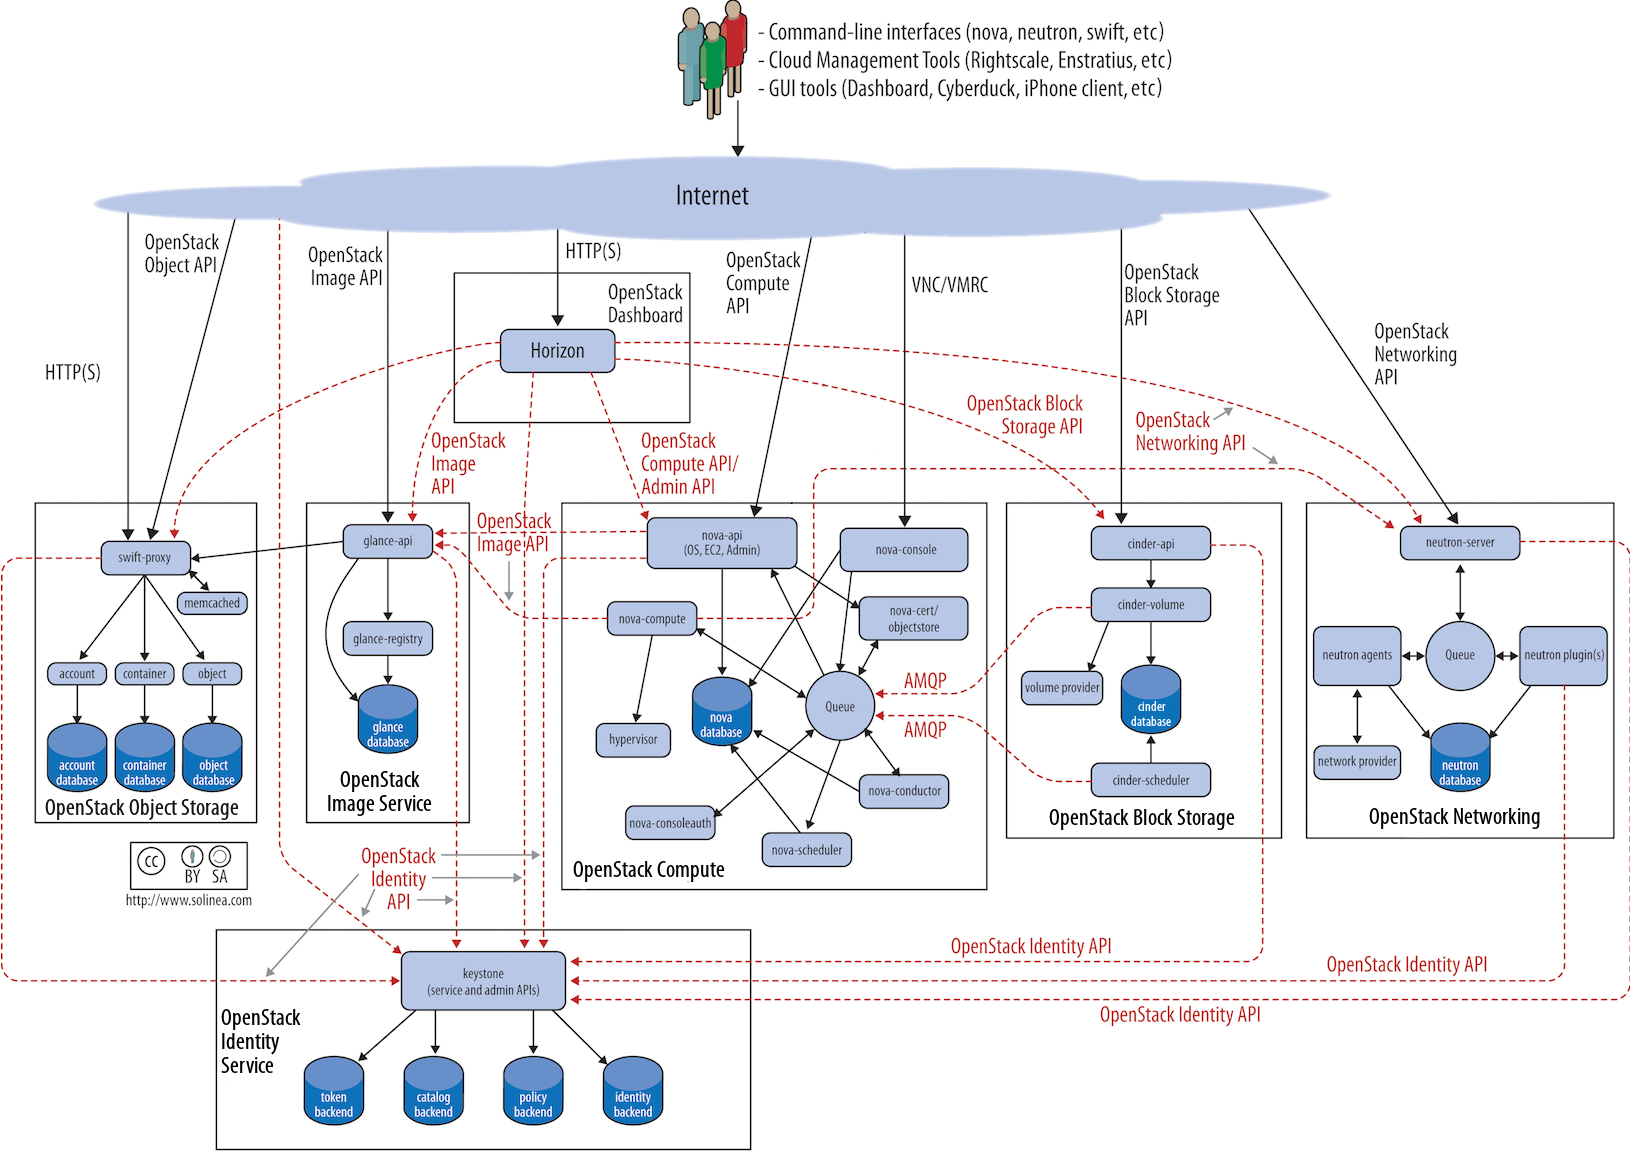
\includegraphics[width=.9\linewidth]{./openstack-detailed.png}
\end{center}
\end{frame}

\begin{frame}[label={sec:org83a3ae9}]{Containers}
\begin{itemize}
\item Docker
\item LXC
\item OpenVZ
\item chroot
\end{itemize}
\end{frame}

\begin{frame}[label={sec:org79d80fb}]{Recap}
\begin{itemize}
\item Why we should use virtualization?
\item What types of hypervisors we know? Any examples?
\item Name some projects that uses or build on top of hypervisor technologies.
\end{itemize}
\end{frame}
\end{document}
